\section{Discussion}
\begin{marginfigure}
	\vspace{-8cm}	
	\centering
	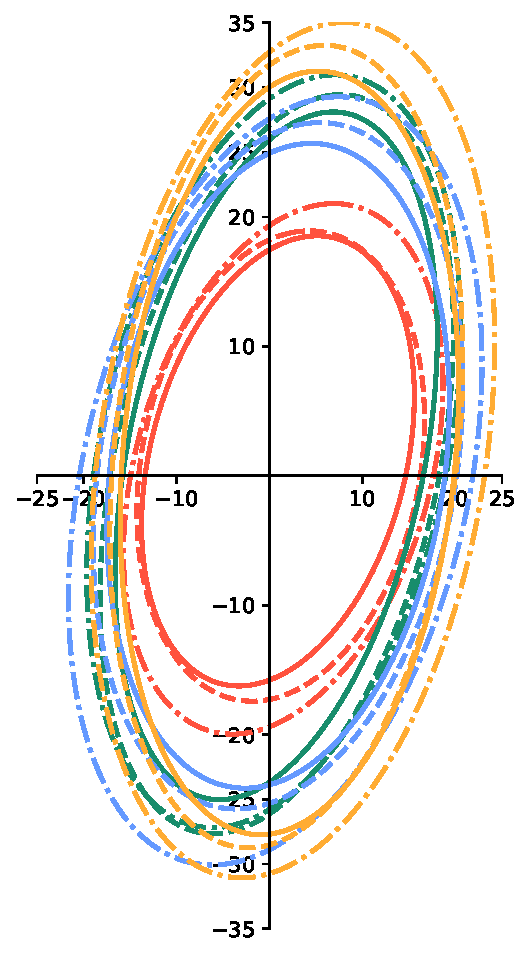
\includegraphics[height=\linewidth]{ellipses_single}
	\caption{Elliptic envelope plot for single models.\newline}
	\label{fig:ell_single}
\end{marginfigure}
\begin{marginfigure}
	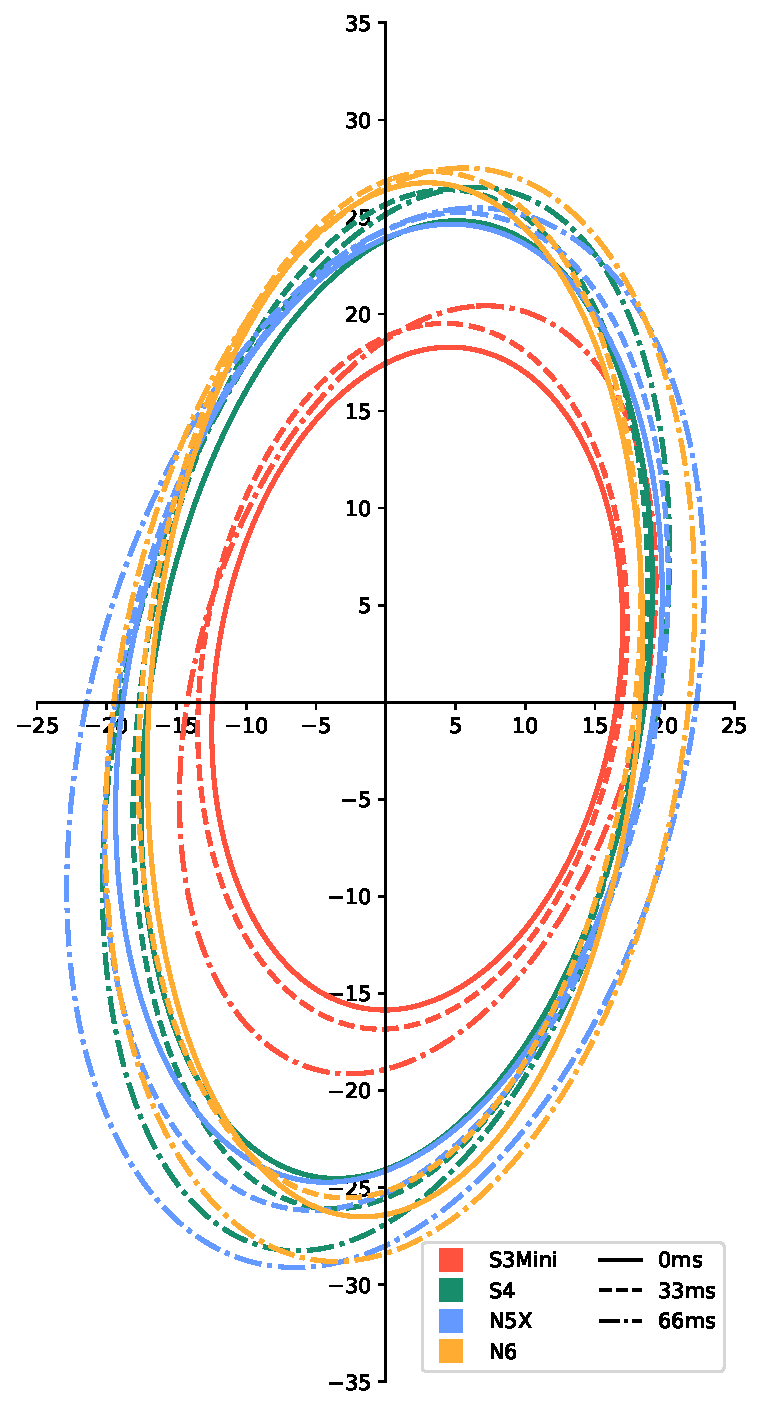
\includegraphics[height=\linewidth]{ellipses_general}
	\caption{Elliptic envelope plot for general models.}
	\label{fig:ell_general}
\end{marginfigure}
Motivated by related work, we conducted a study where participants performed touches on smartphones during which we sampled the internal sensors. 
A combination of a neural network and accelerometer and gyroscope values from the internal sensors allowed us to predict future touches on the smartphone. 
We have focused on showing the possibility of the applicability of our approach as using the IMU is feasible for ordinary usage.

Our results show that touch prediction with neural networks based on internal sensor values is possible, with fairly high precision accuracy.
For increasing prediction times prediction errors increase, e.g. for the N5X the single model for a prediction time of 0ms average prediction errors were $ 17.01mm $ while for 66ms the errors increased to $ 19.96mm $.
This trend can be observed for all telephones, whether single or general model.
Same holds for the elliptic envelope areas where the enclosed area increases for increasing prediction times.
This suggests that the data we collected during our study is either not feasible for predicting touches into the future or that the amount of sensor movement patterns did not differ too much, meaning looking at the times to complete the touches (see \cref{sec:prepro}) participants tried to perform the touches as fast as possible to end the study leading to data consisting of a fairly high amount of fast touches and to an occlusion of slow touches. 
The fact that the general model performed better than the single models might be due to a better generalization of the data, leading to overall lower errors.
To return to the use cases from \cref{sec:intro}, our average errors (single models: 16.67mm$_{0ms}$ (SD = 2.47mm) to 18.82mm$_{66ms}$ (SD = 2.67mm) ; general model: 16.17mm$_{0ms}$ (SD = 1.88mm) to 18.05mm$_{66ms}$ (SD = 2.07mm)) will not allow content to be preloaded which requires clicking small icons or weblinks. 
However, our results could be applied to highlighting larger elements or preloading content from larger elements.

\subsection*{Limitations}
In this paper we focused on one specific use task where users touched randomized targets on smartphones while sitting on a chair without armrests. 
The sensor samples generated during our study are specific for this use case and thereby do not cover ordinary smartphone usage and implied phone movement when e.g. walking, lying in bed, or operating the phone in a train.
An In-The-Wild study is open for future work, where participants are handed out phones which relentlessly record touches and sample the IMU.
The variety of touches during different activities would lead to a more generalizable dataset for touch prediction.
The participants tried to complete the tasks as fast as possible because the study was exhausting for both the hand and the eyes.
This led to a high amount of sensor data from fast touches and a low percentage of slow touches.
Future work could explore the variety of different touches ranging from slow to fast touches  while sampling the IMU.
\begin{margintable}
	\vspace{-7cm}
	\centering
	\begin{tabularx}{1\marginparwidth}{XXd{4.2}d{4.2}d{4.2}}
		
		\toprule
		
		&\textbf{Model}&\multicolumn{1}{c}{\textbf{0ms}}&\multicolumn{1}{c}{\textbf{33ms}}&\multicolumn{1}{c}{\textbf{66ms}} \\
		\midrule
		
		\multirow{2}{*}{\textsc{S3}}   &\multirow{1}{*}{\textbf{S}}  &\cellcolor{green!25}766.92 & \cellcolor{green!25}864.35&1049.42       \\
		\cmidrule{2-5}
		&\multirow{1}{*}{\textbf{G}} &778.93&869.17&\cellcolor{green!25}1002.76     \\
		\midrule		
		\multirow{2}{*}{\textsc{S4}}   &\multirow{1}{*}{\textbf{S}}  &\cellcolor{green!25}1354.96&1588.03&1733.1       \\
		\cmidrule{2-5}
		&\multirow{1}{*}{\textbf{G}} &1376.14&\cellcolor{green!25}1482.92&\cellcolor{green!25}1656.89     \\
		\midrule
		\multirow{2}{*}{\textsc{N5X}}  &\multirow{1}{*}{\textbf{S}}  &\cellcolor{green!25}1413.76&1612.83&1972.12       \\
		\cmidrule{2-5}
		&\multirow{1}{*}{\textbf{G}} &1477.92&\cellcolor{green!25}1573.48&\cellcolor{green!25}1871.57     \\
		\midrule
		\multirow{2}{*}{\textsc{N6}}   &\multirow{1}{*}{\textbf{S}}  &1661.86&1814.29&2176.2       \\
		\cmidrule{2-5}
		&\multirow{1}{*}{\textbf{G}}&\cellcolor{green!25}1462.5&\cellcolor{green!25}1479.93&\cellcolor{green!25}1826.55\\							         		
		\bottomrule    
	\end{tabularx}%
	\caption[Ellipse areas]{\small Ellipse areas ($ mm^{2} $) from single models seen in \cref{fig:ell_single} and from general models seen in \cref{fig:ell_general}.}
	\label{tab:areas}
\end{margintable}
